\section{Zustandsraumdarstellung eines Wissensverarbeitungsproblems}

Die vier wichtigsten Komponenten f�r so ein System, die man kennen muss, sind Fakten, Regeln und Anfragen. 

\textbf{Fakten} sind Eintr�ge in der Fakten- oder Datenbasis. F�r jedes Problem beginnt das System mit einer Beschreibung des gesamten bekannten Wissens �ber eine Problemstellung. 

\textbf{Regeln} werden verwendet, um einen L�sungsschritt zu erzeugen. Mit Hilfe von Regeln werden neue Fakten ber�cksichtigt und einige fr�here verworfen. Das bedeutet, dass die Faktenbasis durch die Anwendung von Regeln ver�ndert wird.

\textbf{Anfragen}, die als Pr�dikate konstruiert sind, beschreiben die Bedingungen, die ein Problem umgeben. Wenn das Pr�dikat in der Datenbasis gefunden wird (nachdem Fakten einige Regeln durchlaufen haben), ist das Problem gel�st.  

Eine �bersicht �ber die Beziehungen zwischen diesen drei Komponenten ist in Abbildung~\ref{fig:xps-relationships} dargestellt.

\begin{figure}[H]
    \centering
    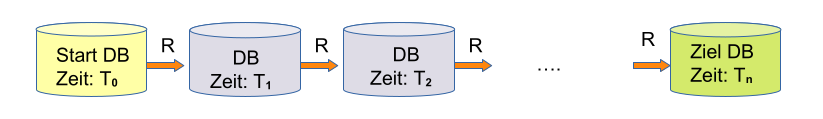
\includegraphics[width=\textwidth]{figures/kap7/state-space-of-xps.png}
    \caption{Beziehung zwischen Fakten, Regeln und Abfragen}
    \label{fig:xps-relationships}
\end{figure}

Dabei ist es wichtig zu beachten, dass der Zustandsraum nicht definiert, wie ein Problem mit den Regeln gel�st werden kann. Hierf�r ist eine Suchfunktion erforderlich.